\documentclass{standalone}
\usepackage{tikz}
\usetikzlibrary{patterns, positioning}


\begin{document}
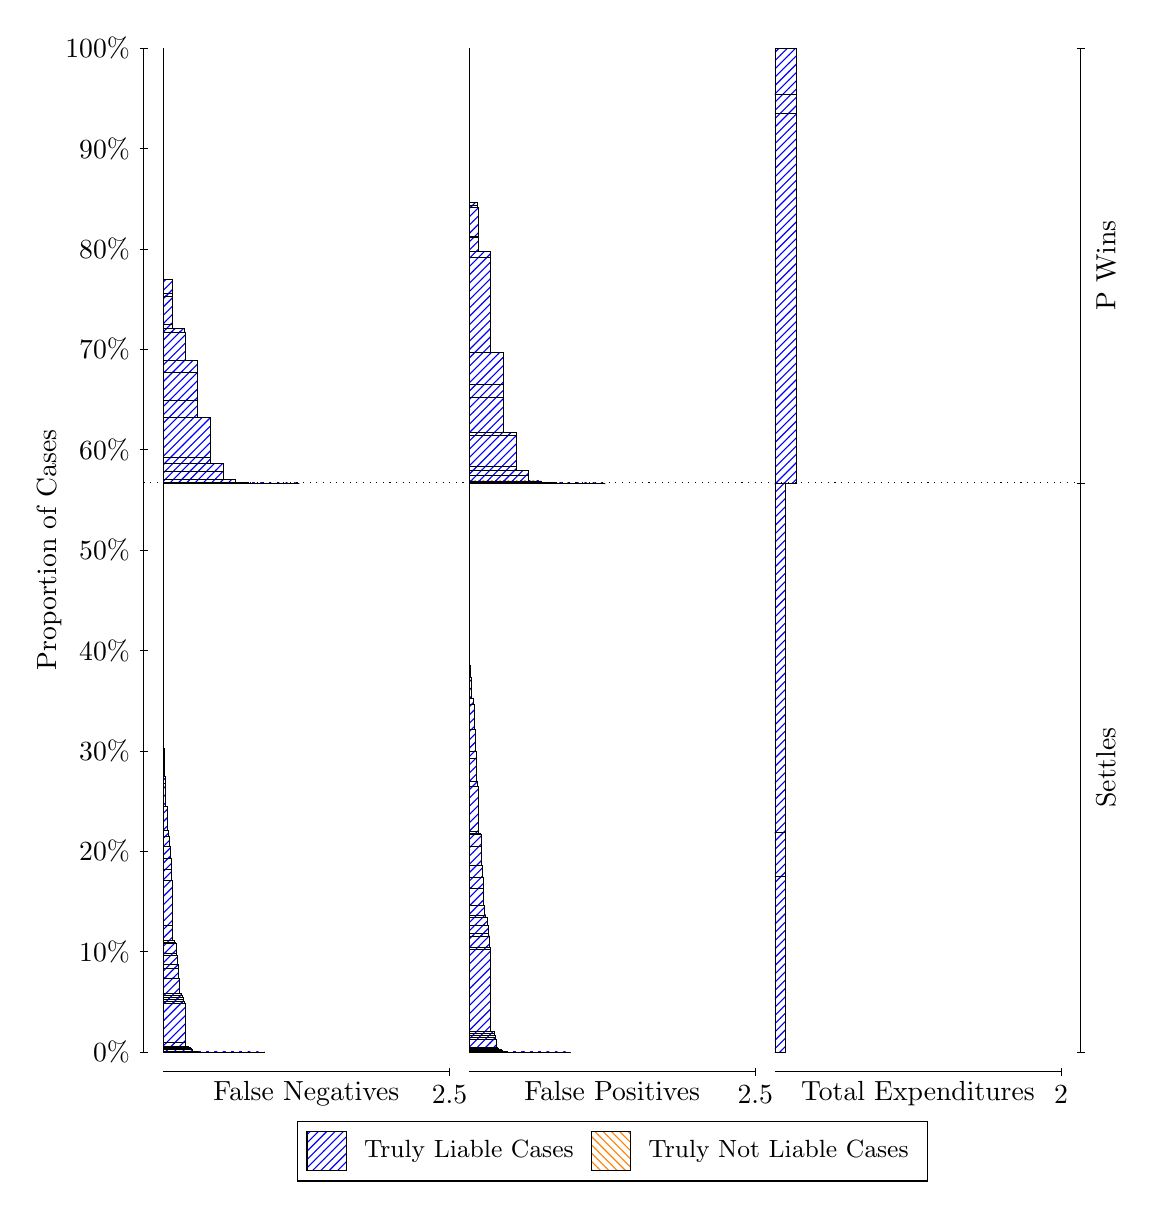
\begin{tikzpicture}
\draw[black, very thin] (1.5,1.75) -- (1.5,14.5);
\node[rotate=90, text=black, anchor=center] at (0.3, 8.125) {Proportion of Cases};
\draw[black, very thin] (1.45,1.75) -- (1.55,1.75);
\node[text=black, anchor=east] at (1.45, 1.75) {0\%};
\draw[black, very thin] (1.45,3.025) -- (1.55,3.025);
\node[text=black, anchor=east] at (1.45, 3.025) {10\%};
\draw[black, very thin] (1.45,4.3) -- (1.55,4.3);
\node[text=black, anchor=east] at (1.45, 4.3) {20\%};
\draw[black, very thin] (1.45,5.575) -- (1.55,5.575);
\node[text=black, anchor=east] at (1.45, 5.575) {30\%};
\draw[black, very thin] (1.45,6.85) -- (1.55,6.85);
\node[text=black, anchor=east] at (1.45, 6.85) {40\%};
\draw[black, very thin] (1.45,8.125) -- (1.55,8.125);
\node[text=black, anchor=east] at (1.45, 8.125) {50\%};
\draw[black, very thin] (1.45,9.4) -- (1.55,9.4);
\node[text=black, anchor=east] at (1.45, 9.4) {60\%};
\draw[black, very thin] (1.45,10.675) -- (1.55,10.675);
\node[text=black, anchor=east] at (1.45, 10.675) {70\%};
\draw[black, very thin] (1.45,11.95) -- (1.55,11.95);
\node[text=black, anchor=east] at (1.45, 11.95) {80\%};
\draw[black, very thin] (1.45,13.225) -- (1.55,13.225);
\node[text=black, anchor=east] at (1.45, 13.225) {90\%};
\draw[black, very thin] (1.45,14.5) -- (1.55,14.5);
\node[text=black, anchor=east] at (1.45, 14.5) {100\%};

\draw[black, very thin] (13.4,1.75) -- (13.4,14.5);
\draw[black, very thin] (13.35,1.75) -- (13.45,1.75);
\node[anchor=west] at (13.35, 1.75) {};
\draw[black, very thin] (13.35,8.9775) -- (13.45,8.9775);
\node[anchor=west] at (13.35, 8.9775) {};
\draw[black, very thin] (13.35,14.5) -- (13.45,14.5);
\node[anchor=west] at (13.35, 14.5) {};

\draw[black, very thin, pattern color=blue, pattern=north east lines] (1.75,1.75) rectangle (3.0398,1.75);
\draw[black, very thin, pattern color=blue, pattern=north east lines] (1.75,1.75) rectangle (2.9672,1.75);
\draw[black, very thin, pattern color=blue, pattern=north east lines] (1.75,1.75) rectangle (2.8945,1.75);
\draw[black, very thin, pattern color=blue, pattern=north east lines] (1.75,1.75) rectangle (2.8784,1.75);
\draw[black, very thin, pattern color=blue, pattern=north east lines] (1.75,1.75) rectangle (2.8218,1.75);
\draw[black, very thin, pattern color=blue, pattern=north east lines] (1.75,1.75) rectangle (2.8057,1.75);
\draw[black, very thin, pattern color=blue, pattern=north east lines] (1.75,1.75) rectangle (2.7492,1.75);
\draw[black, very thin, pattern color=blue, pattern=north east lines] (1.75,1.75) rectangle (2.733,1.75);
\draw[black, very thin, pattern color=blue, pattern=north east lines] (1.75,1.75) rectangle (2.7169,1.75);
\draw[black, very thin, pattern color=blue, pattern=north east lines] (1.75,1.75) rectangle (2.6765,1.75);
\draw[black, very thin, pattern color=blue, pattern=north east lines] (1.75,1.75) rectangle (2.6604,1.75);
\draw[black, very thin, pattern color=blue, pattern=north east lines] (1.75,1.75) rectangle (2.6442,1.75);
\draw[black, very thin, pattern color=blue, pattern=north east lines] (1.75,1.75) rectangle (2.6038,1.75);
\draw[black, very thin, pattern color=blue, pattern=north east lines] (1.75,1.75) rectangle (2.5877,1.75);
\draw[black, very thin, pattern color=blue, pattern=north east lines] (1.75,1.75) rectangle (2.5715,1.75);
\draw[black, very thin, pattern color=blue, pattern=north east lines] (1.75,1.75) rectangle (2.5554,1.75);
\draw[black, very thin, pattern color=blue, pattern=north east lines] (1.75,1.75) rectangle (2.5312,1.75);
\draw[black, very thin, pattern color=blue, pattern=north east lines] (1.75,1.75) rectangle (2.515,1.75);
\draw[black, very thin, pattern color=blue, pattern=north east lines] (1.75,1.75) rectangle (2.4989,1.75);
\draw[black, very thin, pattern color=blue, pattern=north east lines] (1.75,1.75) rectangle (2.4827,1.75);
\draw[black, very thin, pattern color=blue, pattern=north east lines] (1.75,1.75) rectangle (2.4585,1.75);
\draw[black, very thin, pattern color=blue, pattern=north east lines] (1.75,1.75) rectangle (2.4424,1.75);
\draw[black, very thin, pattern color=blue, pattern=north east lines] (1.75,1.75) rectangle (2.4262,1.75);
\draw[black, very thin, pattern color=blue, pattern=north east lines] (1.75,1.75) rectangle (2.4101,1.75);
\draw[black, very thin, pattern color=blue, pattern=north east lines] (1.75,1.75) rectangle (2.3939,1.75);
\draw[black, very thin, pattern color=blue, pattern=north east lines] (1.75,1.75) rectangle (2.3858,1.75);
\draw[black, very thin, pattern color=blue, pattern=north east lines] (1.75,1.75) rectangle (2.3697,1.75);
\draw[black, very thin, pattern color=blue, pattern=north east lines] (1.75,1.75) rectangle (2.3535,1.75);
\draw[black, very thin, pattern color=blue, pattern=north east lines] (1.75,1.75) rectangle (2.3374,1.75);
\draw[black, very thin, pattern color=blue, pattern=north east lines] (1.75,1.75) rectangle (2.3212,1.75);
\draw[black, very thin, pattern color=blue, pattern=north east lines] (1.75,1.75) rectangle (2.3132,1.75);
\draw[black, very thin, pattern color=blue, pattern=north east lines] (1.75,1.75) rectangle (2.297,1.7501);
\draw[black, very thin, pattern color=blue, pattern=north east lines] (1.75,1.7501) rectangle (2.2809,1.7506);
\draw[black, very thin, pattern color=blue, pattern=north east lines] (1.75,1.7506) rectangle (2.2647,1.7507);
\draw[black, very thin, pattern color=blue, pattern=north east lines] (1.75,1.7507) rectangle (2.2486,1.7508);
\draw[black, very thin, pattern color=blue, pattern=north east lines] (1.75,1.7508) rectangle (2.2405,1.7508);
\draw[black, very thin, pattern color=blue, pattern=north east lines] (1.75,1.7508) rectangle (2.2324,1.7509);
\draw[black, very thin, pattern color=blue, pattern=north east lines] (1.75,1.7509) rectangle (2.2244,1.7509);
\draw[black, very thin, pattern color=blue, pattern=north east lines] (1.75,1.7509) rectangle (2.2082,1.751);
\draw[black, very thin, pattern color=blue, pattern=north east lines] (1.75,1.751) rectangle (2.1921,1.7533);
\draw[black, very thin, pattern color=blue, pattern=north east lines] (1.75,1.7533) rectangle (2.1759,1.754);
\draw[black, very thin, pattern color=blue, pattern=north east lines] (1.75,1.754) rectangle (2.1678,1.7553);
\draw[black, very thin, pattern color=blue, pattern=north east lines] (1.75,1.7553) rectangle (2.1598,1.7558);
\draw[black, very thin, pattern color=blue, pattern=north east lines] (1.75,1.7558) rectangle (2.1517,1.7565);
\draw[black, very thin, pattern color=blue, pattern=north east lines] (1.75,1.7565) rectangle (2.1355,1.7585);
\draw[black, very thin, pattern color=blue, pattern=north east lines] (1.75,1.7585) rectangle (2.1194,1.782);
\draw[black, very thin, pattern color=blue, pattern=north east lines] (1.75,1.782) rectangle (2.1032,1.7914);
\draw[black, very thin, pattern color=blue, pattern=north east lines] (1.75,1.7914) rectangle (2.0952,1.8014);
\draw[black, very thin, pattern color=blue, pattern=north east lines] (1.75,1.8014) rectangle (2.0871,1.808);
\draw[black, very thin, pattern color=blue, pattern=north east lines] (1.75,1.808) rectangle (2.079,1.8101);
\draw[black, very thin, pattern color=blue, pattern=north east lines] (1.75,1.8101) rectangle (2.0709,1.8158);
\draw[black, very thin, pattern color=blue, pattern=north east lines] (1.75,1.8158) rectangle (2.0629,1.8188);
\draw[black, very thin, pattern color=blue, pattern=north east lines] (1.75,1.8188) rectangle (2.0467,1.8218);
\draw[black, very thin, pattern color=blue, pattern=north east lines] (1.75,1.8218) rectangle (2.0306,1.8701);
\draw[black, very thin, pattern color=blue, pattern=north east lines] (1.75,1.8701) rectangle (2.0225,2.3738);
\draw[black, very thin, pattern color=blue, pattern=north east lines] (1.75,2.3738) rectangle (2.0144,2.3974);
\draw[black, very thin, pattern color=blue, pattern=north east lines] (1.75,2.3974) rectangle (2.0064,2.4243);
\draw[black, very thin, pattern color=blue, pattern=north east lines] (1.75,2.4243) rectangle (1.9983,2.4448);
\draw[black, very thin, pattern color=blue, pattern=north east lines] (1.75,2.4448) rectangle (1.9902,2.4661);
\draw[black, very thin, pattern color=blue, pattern=north east lines] (1.75,2.4661) rectangle (1.9741,2.4975);
\draw[black, very thin, pattern color=blue, pattern=north east lines] (1.75,2.4975) rectangle (1.9579,2.6919);
\draw[black, very thin, pattern color=blue, pattern=north east lines] (1.75,2.6919) rectangle (1.9418,2.8147);
\draw[black, very thin, pattern color=blue, pattern=north east lines] (1.75,2.8147) rectangle (1.9337,2.8701);
\draw[black, very thin, pattern color=blue, pattern=north east lines] (1.75,2.8701) rectangle (1.9256,2.9771);
\draw[black, very thin, pattern color=blue, pattern=north east lines] (1.75,2.9771) rectangle (1.9175,3.0071);
\draw[black, very thin, pattern color=blue, pattern=north east lines] (1.75,3.0071) rectangle (1.9095,3.1251);
\draw[black, very thin, pattern color=blue, pattern=north east lines] (1.75,3.1251) rectangle (1.9014,3.1443);
\draw[black, very thin, pattern color=blue, pattern=north east lines] (1.75,3.1443) rectangle (1.8852,3.1635);
\draw[black, very thin, pattern color=blue, pattern=north east lines] (1.75,3.1635) rectangle (1.8691,3.3565);
\draw[black, very thin, pattern color=blue, pattern=north east lines] (1.75,3.3565) rectangle (1.861,3.9278);
\draw[black, very thin, pattern color=blue, pattern=north east lines] (1.75,3.9278) rectangle (1.8529,4.0715);
\draw[black, very thin, pattern color=blue, pattern=north east lines] (1.75,4.0715) rectangle (1.8449,4.2147);
\draw[black, very thin, pattern color=blue, pattern=north east lines] (1.75,4.2147) rectangle (1.8368,4.3641);
\draw[black, very thin, pattern color=blue, pattern=north east lines] (1.75,4.3641) rectangle (1.8287,4.4873);
\draw[black, very thin, pattern color=blue, pattern=north east lines] (1.75,4.4873) rectangle (1.8126,4.5665);
\draw[black, very thin, pattern color=blue, pattern=north east lines] (1.75,4.5665) rectangle (1.7964,4.8762);
\draw[black, very thin, pattern color=blue, pattern=north east lines] (1.75,4.8762) rectangle (1.7803,5.1565);
\draw[black, very thin, pattern color=blue, pattern=north east lines] (1.75,5.1565) rectangle (1.7722,5.2509);
\draw[black, very thin, pattern color=blue, pattern=north east lines] (1.75,5.2509) rectangle (1.7641,5.5345);
\draw[black, very thin, pattern color=blue, pattern=north east lines] (1.75,5.5345) rectangle (1.7561,5.6091);
\draw[black, very thin, pattern color=orange, pattern=north west lines] (1.75,5.6091) rectangle (1.75,5.6091);
\draw[black, very thin, pattern color=blue, pattern=north east lines] (1.75,5.6091) rectangle (1.75,8.9775);
\draw[black, very thin, pattern color=blue, pattern=north east lines] (1.75,8.9775) rectangle (3.4758,8.9775);
\draw[black, very thin, pattern color=blue, pattern=north east lines] (1.75,8.9775) rectangle (3.3144,8.9775);
\draw[black, very thin, pattern color=blue, pattern=north east lines] (1.75,8.9775) rectangle (3.1529,8.9775);
\draw[black, very thin, pattern color=blue, pattern=north east lines] (1.75,8.9775) rectangle (3.1529,8.9775);
\draw[black, very thin, pattern color=blue, pattern=north east lines] (1.75,8.9775) rectangle (2.9914,8.9777);
\draw[black, very thin, pattern color=blue, pattern=north east lines] (1.75,8.9777) rectangle (2.9914,8.9779);
\draw[black, very thin, pattern color=blue, pattern=north east lines] (1.75,8.9779) rectangle (2.8299,8.9831);
\draw[black, very thin, pattern color=blue, pattern=north east lines] (1.75,8.9831) rectangle (2.8259,8.9831);
\draw[black, very thin, pattern color=blue, pattern=north east lines] (1.75,8.9831) rectangle (2.6684,9.0237);
\draw[black, very thin, pattern color=blue, pattern=north east lines] (1.75,9.0237) rectangle (2.6644,9.0237);
\draw[black, very thin, pattern color=blue, pattern=north east lines] (1.75,9.0237) rectangle (2.5069,9.126);
\draw[black, very thin, pattern color=blue, pattern=north east lines] (1.75,9.126) rectangle (2.5069,9.2229);
\draw[black, very thin, pattern color=blue, pattern=north east lines] (1.75,9.2229) rectangle (2.5029,9.2229);
\draw[black, very thin, pattern color=blue, pattern=north east lines] (1.75,9.2229) rectangle (2.5029,9.2229);
\draw[black, very thin, pattern color=blue, pattern=north east lines] (1.75,9.2229) rectangle (2.3455,9.3032);
\draw[black, very thin, pattern color=blue, pattern=north east lines] (1.75,9.3032) rectangle (2.3455,9.8132);
\draw[black, very thin, pattern color=blue, pattern=north east lines] (1.75,9.8132) rectangle (2.3414,9.8132);
\draw[black, very thin, pattern color=blue, pattern=north east lines] (1.75,9.8132) rectangle (2.3414,9.8132);
\draw[black, very thin, pattern color=blue, pattern=north east lines] (1.75,9.8132) rectangle (2.184,10.031);
\draw[black, very thin, pattern color=blue, pattern=north east lines] (1.75,10.031) rectangle (2.184,10.387);
\draw[black, very thin, pattern color=blue, pattern=north east lines] (1.75,10.387) rectangle (2.184,10.534);
\draw[black, very thin, pattern color=blue, pattern=north east lines] (1.75,10.534) rectangle (2.1799,10.535);
\draw[black, very thin, pattern color=blue, pattern=north east lines] (1.75,10.535) rectangle (2.1799,10.535);
\draw[black, very thin, pattern color=blue, pattern=north east lines] (1.75,10.535) rectangle (2.1799,10.535);
\draw[black, very thin, pattern color=blue, pattern=north east lines] (1.75,10.535) rectangle (2.0225,10.895);
\draw[black, very thin, pattern color=blue, pattern=north east lines] (1.75,10.895) rectangle (2.0185,10.896);
\draw[black, very thin, pattern color=blue, pattern=north east lines] (1.75,10.896) rectangle (2.0185,10.941);
\draw[black, very thin, pattern color=blue, pattern=north east lines] (1.75,10.941) rectangle (1.861,10.942);
\draw[black, very thin, pattern color=blue, pattern=north east lines] (1.75,10.942) rectangle (1.861,10.996);
\draw[black, very thin, pattern color=blue, pattern=north east lines] (1.75,10.996) rectangle (1.861,10.997);
\draw[black, very thin, pattern color=blue, pattern=north east lines] (1.75,10.997) rectangle (1.857,11.351);
\draw[black, very thin, pattern color=blue, pattern=north east lines] (1.75,11.351) rectangle (1.857,11.385);
\draw[black, very thin, pattern color=blue, pattern=north east lines] (1.75,11.385) rectangle (1.857,11.562);
\draw[black, very thin, pattern color=orange, pattern=north west lines] (1.75,11.562) rectangle (1.75,11.562);
\draw[black, very thin, pattern color=blue, pattern=north east lines] (1.75,11.562) rectangle (1.75,14.5);
\draw[black, very thin, pattern color=orange, pattern=north west lines] (5.6333,1.75) rectangle (6.9232,1.75);
\draw[black, very thin, pattern color=blue, pattern=north east lines] (5.6333,1.75) rectangle (6.9232,1.75);
\draw[black, very thin, pattern color=orange, pattern=north west lines] (5.6333,1.75) rectangle (6.8505,1.75);
\draw[black, very thin, pattern color=blue, pattern=north east lines] (5.6333,1.75) rectangle (6.8505,1.75);
\draw[black, very thin, pattern color=orange, pattern=north west lines] (5.6333,1.75) rectangle (6.7778,1.75);
\draw[black, very thin, pattern color=blue, pattern=north east lines] (5.6333,1.75) rectangle (6.7778,1.75);
\draw[black, very thin, pattern color=blue, pattern=north east lines] (5.6333,1.75) rectangle (6.7617,1.75);
\draw[black, very thin, pattern color=orange, pattern=north west lines] (5.6333,1.75) rectangle (6.7052,1.75);
\draw[black, very thin, pattern color=blue, pattern=north east lines] (5.6333,1.75) rectangle (6.7052,1.75);
\draw[black, very thin, pattern color=blue, pattern=north east lines] (5.6333,1.75) rectangle (6.689,1.75);
\draw[black, very thin, pattern color=orange, pattern=north west lines] (5.6333,1.75) rectangle (6.6325,1.75);
\draw[black, very thin, pattern color=blue, pattern=north east lines] (5.6333,1.75) rectangle (6.6325,1.75);
\draw[black, very thin, pattern color=blue, pattern=north east lines] (5.6333,1.75) rectangle (6.6164,1.75);
\draw[black, very thin, pattern color=blue, pattern=north east lines] (5.6333,1.75) rectangle (6.6002,1.75);
\draw[black, very thin, pattern color=orange, pattern=north west lines] (5.6333,1.75) rectangle (6.5598,1.75);
\draw[black, very thin, pattern color=blue, pattern=north east lines] (5.6333,1.75) rectangle (6.5598,1.75);
\draw[black, very thin, pattern color=blue, pattern=north east lines] (5.6333,1.75) rectangle (6.5437,1.75);
\draw[black, very thin, pattern color=blue, pattern=north east lines] (5.6333,1.75) rectangle (6.5275,1.75);
\draw[black, very thin, pattern color=orange, pattern=north west lines] (5.6333,1.75) rectangle (6.4872,1.75);
\draw[black, very thin, pattern color=blue, pattern=north east lines] (5.6333,1.75) rectangle (6.4872,1.75);
\draw[black, very thin, pattern color=blue, pattern=north east lines] (5.6333,1.75) rectangle (6.471,1.75);
\draw[black, very thin, pattern color=blue, pattern=north east lines] (5.6333,1.75) rectangle (6.4549,1.75);
\draw[black, very thin, pattern color=blue, pattern=north east lines] (5.6333,1.75) rectangle (6.4387,1.75);
\draw[black, very thin, pattern color=orange, pattern=north west lines] (5.6333,1.75) rectangle (6.4145,1.75);
\draw[black, very thin, pattern color=blue, pattern=north east lines] (5.6333,1.75) rectangle (6.4145,1.75);
\draw[black, very thin, pattern color=blue, pattern=north east lines] (5.6333,1.75) rectangle (6.3984,1.75);
\draw[black, very thin, pattern color=blue, pattern=north east lines] (5.6333,1.75) rectangle (6.3822,1.75);
\draw[black, very thin, pattern color=blue, pattern=north east lines] (5.6333,1.75) rectangle (6.3661,1.75);
\draw[black, very thin, pattern color=orange, pattern=north west lines] (5.6333,1.75) rectangle (6.3418,1.75);
\draw[black, very thin, pattern color=blue, pattern=north east lines] (5.6333,1.75) rectangle (6.3418,1.75);
\draw[black, very thin, pattern color=blue, pattern=north east lines] (5.6333,1.75) rectangle (6.3257,1.75);
\draw[black, very thin, pattern color=blue, pattern=north east lines] (5.6333,1.75) rectangle (6.3095,1.75);
\draw[black, very thin, pattern color=blue, pattern=north east lines] (5.6333,1.75) rectangle (6.2934,1.75);
\draw[black, very thin, pattern color=blue, pattern=north east lines] (5.6333,1.75) rectangle (6.2772,1.75);
\draw[black, very thin, pattern color=orange, pattern=north west lines] (5.6333,1.75) rectangle (6.2692,1.75);
\draw[black, very thin, pattern color=blue, pattern=north east lines] (5.6333,1.75) rectangle (6.2692,1.75);
\draw[black, very thin, pattern color=blue, pattern=north east lines] (5.6333,1.75) rectangle (6.253,1.75);
\draw[black, very thin, pattern color=blue, pattern=north east lines] (5.6333,1.75) rectangle (6.2369,1.75);
\draw[black, very thin, pattern color=blue, pattern=north east lines] (5.6333,1.75) rectangle (6.2207,1.75);
\draw[black, very thin, pattern color=blue, pattern=north east lines] (5.6333,1.75) rectangle (6.2046,1.75);
\draw[black, very thin, pattern color=orange, pattern=north west lines] (5.6333,1.75) rectangle (6.1965,1.75);
\draw[black, very thin, pattern color=blue, pattern=north east lines] (5.6333,1.75) rectangle (6.1965,1.7502);
\draw[black, very thin, pattern color=blue, pattern=north east lines] (5.6333,1.7502) rectangle (6.1804,1.7502);
\draw[black, very thin, pattern color=blue, pattern=north east lines] (5.6333,1.7502) rectangle (6.1642,1.7503);
\draw[black, very thin, pattern color=blue, pattern=north east lines] (5.6333,1.7503) rectangle (6.1481,1.7507);
\draw[black, very thin, pattern color=blue, pattern=north east lines] (5.6333,1.7507) rectangle (6.1319,1.7512);
\draw[black, very thin, pattern color=orange, pattern=north west lines] (5.6333,1.7512) rectangle (6.1238,1.7512);
\draw[black, very thin, pattern color=blue, pattern=north east lines] (5.6333,1.7512) rectangle (6.1238,1.7526);
\draw[black, very thin, pattern color=blue, pattern=north east lines] (5.6333,1.7526) rectangle (6.1158,1.7531);
\draw[black, very thin, pattern color=blue, pattern=north east lines] (5.6333,1.7531) rectangle (6.1077,1.7537);
\draw[black, very thin, pattern color=blue, pattern=north east lines] (5.6333,1.7537) rectangle (6.0915,1.7538);
\draw[black, very thin, pattern color=blue, pattern=north east lines] (5.6333,1.7538) rectangle (6.0754,1.7538);
\draw[black, very thin, pattern color=blue, pattern=north east lines] (5.6333,1.7538) rectangle (6.0592,1.7557);
\draw[black, very thin, pattern color=orange, pattern=north west lines] (5.6333,1.7557) rectangle (6.0512,1.7557);
\draw[black, very thin, pattern color=blue, pattern=north east lines] (5.6333,1.7557) rectangle (6.0512,1.7754);
\draw[black, very thin, pattern color=blue, pattern=north east lines] (5.6333,1.7754) rectangle (6.0431,1.7773);
\draw[black, very thin, pattern color=blue, pattern=north east lines] (5.6333,1.7773) rectangle (6.035,1.7849);
\draw[black, very thin, pattern color=blue, pattern=north east lines] (5.6333,1.7849) rectangle (6.0189,1.7902);
\draw[black, very thin, pattern color=blue, pattern=north east lines] (5.6333,1.7902) rectangle (6.0027,1.7922);
\draw[black, very thin, pattern color=blue, pattern=north east lines] (5.6333,1.7922) rectangle (5.9866,1.811);
\draw[black, very thin, pattern color=orange, pattern=north west lines] (5.6333,1.811) rectangle (5.9785,1.811);
\draw[black, very thin, pattern color=blue, pattern=north east lines] (5.6333,1.811) rectangle (5.9785,1.9119);
\draw[black, very thin, pattern color=blue, pattern=north east lines] (5.6333,1.9119) rectangle (5.9704,1.9336);
\draw[black, very thin, pattern color=blue, pattern=north east lines] (5.6333,1.9336) rectangle (5.9624,1.9607);
\draw[black, very thin, pattern color=blue, pattern=north east lines] (5.6333,1.9607) rectangle (5.9543,1.9864);
\draw[black, very thin, pattern color=blue, pattern=north east lines] (5.6333,1.9864) rectangle (5.9462,2.0073);
\draw[black, very thin, pattern color=blue, pattern=north east lines] (5.6333,2.0073) rectangle (5.9301,2.0103);
\draw[black, very thin, pattern color=blue, pattern=north east lines] (5.6333,2.0103) rectangle (5.9139,2.0133);
\draw[black, very thin, pattern color=orange, pattern=north west lines] (5.6333,2.0133) rectangle (5.9058,2.0133);
\draw[black, very thin, pattern color=blue, pattern=north east lines] (5.6333,2.0133) rectangle (5.9058,3.0538);
\draw[black, very thin, pattern color=blue, pattern=north east lines] (5.6333,3.0538) rectangle (5.8978,3.0834);
\draw[black, very thin, pattern color=blue, pattern=north east lines] (5.6333,3.0834) rectangle (5.8897,3.2243);
\draw[black, very thin, pattern color=blue, pattern=north east lines] (5.6333,3.2243) rectangle (5.8816,3.2569);
\draw[black, very thin, pattern color=blue, pattern=north east lines] (5.6333,3.2569) rectangle (5.8735,3.3652);
\draw[black, very thin, pattern color=blue, pattern=north east lines] (5.6333,3.3652) rectangle (5.8574,3.4603);
\draw[black, very thin, pattern color=blue, pattern=north east lines] (5.6333,3.4603) rectangle (5.8412,3.4917);
\draw[black, very thin, pattern color=blue, pattern=north east lines] (5.6333,3.4917) rectangle (5.8251,3.6117);
\draw[black, very thin, pattern color=blue, pattern=north east lines] (5.6333,3.6117) rectangle (5.817,3.8327);
\draw[black, very thin, pattern color=blue, pattern=north east lines] (5.6333,3.8327) rectangle (5.8089,3.9713);
\draw[black, very thin, pattern color=blue, pattern=north east lines] (5.6333,3.9713) rectangle (5.8009,4.1168);
\draw[black, very thin, pattern color=blue, pattern=north east lines] (5.6333,4.1168) rectangle (5.7928,4.3606);
\draw[black, very thin, pattern color=blue, pattern=north east lines] (5.6333,4.3606) rectangle (5.7847,4.5088);
\draw[black, very thin, pattern color=blue, pattern=north east lines] (5.6333,4.5088) rectangle (5.7686,4.528);
\draw[black, very thin, pattern color=blue, pattern=north east lines] (5.6333,4.528) rectangle (5.7524,4.5471);
\draw[black, very thin, pattern color=blue, pattern=north east lines] (5.6333,4.5471) rectangle (5.7444,5.1184);
\draw[black, very thin, pattern color=blue, pattern=north east lines] (5.6333,5.1184) rectangle (5.7363,5.1929);
\draw[black, very thin, pattern color=blue, pattern=north east lines] (5.6333,5.1929) rectangle (5.7282,5.4766);
\draw[black, very thin, pattern color=blue, pattern=north east lines] (5.6333,5.4766) rectangle (5.7201,5.5709);
\draw[black, very thin, pattern color=blue, pattern=north east lines] (5.6333,5.5709) rectangle (5.7121,5.8512);
\draw[black, very thin, pattern color=blue, pattern=north east lines] (5.6333,5.8512) rectangle (5.6959,6.1609);
\draw[black, very thin, pattern color=blue, pattern=north east lines] (5.6333,6.1609) rectangle (5.6798,6.2401);
\draw[black, very thin, pattern color=blue, pattern=north east lines] (5.6333,6.2401) rectangle (5.6636,6.3633);
\draw[black, very thin, pattern color=blue, pattern=north east lines] (5.6333,6.3633) rectangle (5.6555,6.5128);
\draw[black, very thin, pattern color=blue, pattern=north east lines] (5.6333,6.5128) rectangle (5.6475,6.6559);
\draw[black, very thin, pattern color=blue, pattern=north east lines] (5.6333,6.6559) rectangle (5.6394,6.7997);
\draw[black, very thin, pattern color=blue, pattern=north east lines] (5.6333,6.7997) rectangle (5.6333,8.9775);
\draw[black, very thin, pattern color=orange, pattern=north west lines] (5.6333,8.9775) rectangle (7.3592,8.9775);
\draw[black, very thin, pattern color=blue, pattern=north east lines] (5.6333,8.9775) rectangle (7.3592,8.9775);
\draw[black, very thin, pattern color=orange, pattern=north west lines] (5.6333,8.9775) rectangle (7.1977,8.9775);
\draw[black, very thin, pattern color=blue, pattern=north east lines] (5.6333,8.9775) rectangle (7.1977,8.9775);
\draw[black, very thin, pattern color=orange, pattern=north west lines] (5.6333,8.9775) rectangle (7.0362,8.9775);
\draw[black, very thin, pattern color=blue, pattern=north east lines] (5.6333,8.9775) rectangle (7.0362,8.9775);
\draw[black, very thin, pattern color=blue, pattern=north east lines] (5.6333,8.9775) rectangle (7.0362,8.9775);
\draw[black, very thin, pattern color=blue, pattern=north east lines] (5.6333,8.9775) rectangle (6.8747,8.9776);
\draw[black, very thin, pattern color=orange, pattern=north west lines] (5.6333,8.9776) rectangle (6.8747,8.9776);
\draw[black, very thin, pattern color=blue, pattern=north east lines] (5.6333,8.9776) rectangle (6.8747,8.9776);
\draw[black, very thin, pattern color=orange, pattern=north west lines] (5.6333,8.9776) rectangle (6.7132,8.9776);
\draw[black, very thin, pattern color=blue, pattern=north east lines] (5.6333,8.9776) rectangle (6.7132,8.9801);
\draw[black, very thin, pattern color=orange, pattern=north west lines] (5.6333,8.9801) rectangle (6.7092,8.9801);
\draw[black, very thin, pattern color=blue, pattern=north east lines] (5.6333,8.9801) rectangle (6.7092,8.9801);
\draw[black, very thin, pattern color=orange, pattern=north west lines] (5.6333,8.9801) rectangle (6.5518,8.9801);
\draw[black, very thin, pattern color=blue, pattern=north east lines] (5.6333,8.9801) rectangle (6.5518,9.0035);
\draw[black, very thin, pattern color=orange, pattern=north west lines] (5.6333,9.0035) rectangle (6.5477,9.0035);
\draw[black, very thin, pattern color=blue, pattern=north east lines] (5.6333,9.0035) rectangle (6.5477,9.0035);
\draw[black, very thin, pattern color=blue, pattern=north east lines] (5.6333,9.0035) rectangle (6.3903,9.0726);
\draw[black, very thin, pattern color=orange, pattern=north west lines] (5.6333,9.0726) rectangle (6.3903,9.0726);
\draw[black, very thin, pattern color=blue, pattern=north east lines] (5.6333,9.0726) rectangle (6.3903,9.1389);
\draw[black, very thin, pattern color=orange, pattern=north west lines] (5.6333,9.1389) rectangle (6.3862,9.1389);
\draw[black, very thin, pattern color=blue, pattern=north east lines] (5.6333,9.1389) rectangle (6.3862,9.1389);
\draw[black, very thin, pattern color=blue, pattern=north east lines] (5.6333,9.1389) rectangle (6.3862,9.1389);
\draw[black, very thin, pattern color=blue, pattern=north east lines] (5.6333,9.1389) rectangle (6.2288,9.1914);
\draw[black, very thin, pattern color=orange, pattern=north west lines] (5.6333,9.1914) rectangle (6.2288,9.1914);
\draw[black, very thin, pattern color=blue, pattern=north east lines] (5.6333,9.1914) rectangle (6.2288,9.5796);
\draw[black, very thin, pattern color=blue, pattern=north east lines] (5.6333,9.5796) rectangle (6.2288,9.6199);
\draw[black, very thin, pattern color=blue, pattern=north east lines] (5.6333,9.6199) rectangle (6.2248,9.6199);
\draw[black, very thin, pattern color=orange, pattern=north west lines] (5.6333,9.6199) rectangle (6.2248,9.6199);
\draw[black, very thin, pattern color=blue, pattern=north east lines] (5.6333,9.6199) rectangle (6.2248,9.6199);
\draw[black, very thin, pattern color=blue, pattern=north east lines] (5.6333,9.6199) rectangle (6.0673,10.059);
\draw[black, very thin, pattern color=blue, pattern=north east lines] (5.6333,10.059) rectangle (6.0673,10.224);
\draw[black, very thin, pattern color=blue, pattern=north east lines] (5.6333,10.224) rectangle (6.0673,10.634);
\draw[black, very thin, pattern color=blue, pattern=north east lines] (5.6333,10.634) rectangle (6.0633,10.634);
\draw[black, very thin, pattern color=orange, pattern=north west lines] (5.6333,10.634) rectangle (6.0633,10.634);
\draw[black, very thin, pattern color=blue, pattern=north east lines] (5.6333,10.634) rectangle (6.0633,10.634);
\draw[black, very thin, pattern color=blue, pattern=north east lines] (5.6333,10.634) rectangle (5.9058,11.838);
\draw[black, very thin, pattern color=blue, pattern=north east lines] (5.6333,11.838) rectangle (5.9058,11.915);
\draw[black, very thin, pattern color=blue, pattern=north east lines] (5.6333,11.915) rectangle (5.9018,11.915);
\draw[black, very thin, pattern color=orange, pattern=north west lines] (5.6333,11.915) rectangle (5.9018,11.915);
\draw[black, very thin, pattern color=blue, pattern=north east lines] (5.6333,11.915) rectangle (5.9018,11.915);
\draw[black, very thin, pattern color=blue, pattern=north east lines] (5.6333,11.915) rectangle (5.7444,12.093);
\draw[black, very thin, pattern color=blue, pattern=north east lines] (5.6333,12.093) rectangle (5.7444,12.11);
\draw[black, very thin, pattern color=blue, pattern=north east lines] (5.6333,12.11) rectangle (5.7444,12.481);
\draw[black, very thin, pattern color=blue, pattern=north east lines] (5.6333,12.481) rectangle (5.7403,12.482);
\draw[black, very thin, pattern color=blue, pattern=north east lines] (5.6333,12.482) rectangle (5.7403,12.498);
\draw[black, very thin, pattern color=orange, pattern=north west lines] (5.6333,12.498) rectangle (5.7403,12.498);
\draw[black, very thin, pattern color=blue, pattern=north east lines] (5.6333,12.498) rectangle (5.7403,12.536);
\draw[black, very thin, pattern color=blue, pattern=north east lines] (5.6333,12.536) rectangle (5.7403,12.537);
\draw[black, very thin, pattern color=orange, pattern=north west lines] (5.6333,12.537) rectangle (5.6333,12.537);
\draw[black, very thin, pattern color=blue, pattern=north east lines] (5.6333,12.537) rectangle (5.6333,14.5);
\draw[black, very thin, pattern color=orange, pattern=north west lines] (9.5167,1.75) rectangle (9.6529,1.75);
\draw[black, very thin, pattern color=blue, pattern=north east lines] (9.5167,1.75) rectangle (9.6529,3.978);
\draw[black, very thin, pattern color=orange, pattern=north west lines] (9.5167,3.978) rectangle (9.6529,3.978);
\draw[black, very thin, pattern color=blue, pattern=north east lines] (9.5167,3.978) rectangle (9.6529,4.5361);
\draw[black, very thin, pattern color=orange, pattern=north west lines] (9.5167,4.5361) rectangle (9.6529,4.5361);
\draw[black, very thin, pattern color=blue, pattern=north east lines] (9.5167,4.5361) rectangle (9.6529,8.9775);
\draw[black, very thin, pattern color=orange, pattern=north west lines] (9.5167,8.9775) rectangle (9.7892,8.9775);
\draw[black, very thin, pattern color=blue, pattern=north east lines] (9.5167,8.9775) rectangle (9.7892,13.671);
\draw[black, very thin, pattern color=orange, pattern=north west lines] (9.5167,13.671) rectangle (9.7892,13.671);
\draw[black, very thin, pattern color=blue, pattern=north east lines] (9.5167,13.671) rectangle (9.7892,13.907);
\draw[black, very thin, pattern color=orange, pattern=north west lines] (9.5167,13.907) rectangle (9.7892,13.907);
\draw[black, very thin, pattern color=blue, pattern=north east lines] (9.5167,13.907) rectangle (9.7892,14.5);
\draw[black, dotted] (1.5,8.9775) -- (13.4,8.9775);
\draw[black, very thin] (1.75,1.5) -- (5.3833,1.5);
\node[text=black, anchor=north] at (3.5667, 1.5) {False Negatives};
\draw[black, very thin] (5.3833,1.45) -- (5.3833,1.55);
\node[text=black, anchor=north] at (5.3833, 1.45) {2.5};

\draw[black, very thin] (5.6333,1.5) -- (9.2667,1.5);
\node[text=black, anchor=north] at (7.45, 1.5) {False Positives};
\draw[black, very thin] (9.2667,1.45) -- (9.2667,1.55);
\node[text=black, anchor=north] at (9.2667, 1.45) {2.5};

\draw[black, very thin] (9.5167,1.5) -- (13.15,1.5);
\node[text=black, anchor=north] at (11.333, 1.5) {Total Expenditures};
\draw[black, very thin] (13.15,1.45) -- (13.15,1.55);
\node[text=black, anchor=north] at (13.15, 1.45) {2};

\node[text=black, centered, rotate=90] at (13.72, 5.3637) {Settles};
\node[text=black, centered, rotate=90] at (13.72, 11.739) {P Wins};

\draw (7.449999999999999,1.5) node[draw=none] (baseCoordinate) {};
\begin{scope}[align=center]
        \matrix[scale=0.5, draw=black, below=0.5cm of baseCoordinate, nodes={draw}, column sep=0.1cm]{
            \node[rectangle, draw, minimum width=0.5cm, minimum height=0.5cm, pattern color=blue, pattern=north east lines] {}; &
            \node[draw=none, font=\small, text=black] (B) {Truly Liable Cases}; &
            \node[rectangle, draw, minimum width=0.5cm, minimum height=0.5cm, pattern color=orange, pattern=north west lines] {}; &
            \node[draw=none, font=\small, text=black] (B) {Truly Not Liable Cases}; \\
            };
\end{scope}

\end{tikzpicture}
\end{document}